\section{Turtledove}
\label{sec:design-turtledove}

Turtledove is an all-in-one solution to ``Tool assisted programming in SML with
special emphasis on semi-automatic rewriting to predefined standard forms''. As
of this writing no integrated development environment exists for SML that offers
high level assistance such as ``refactoring'' or ``go to definition''.
Turtledove is an aim at being the first a back end system that can easily be
integrated into most of the currently available development environments.

To facilitate this Turtledove should be a modular system with a few key tools
described below. At the core of turtledove are the parsers (SML, MLB and Rules),
which makes it possible for the tools to work on any user code.

\begin{figure}[h!]
  \centering
 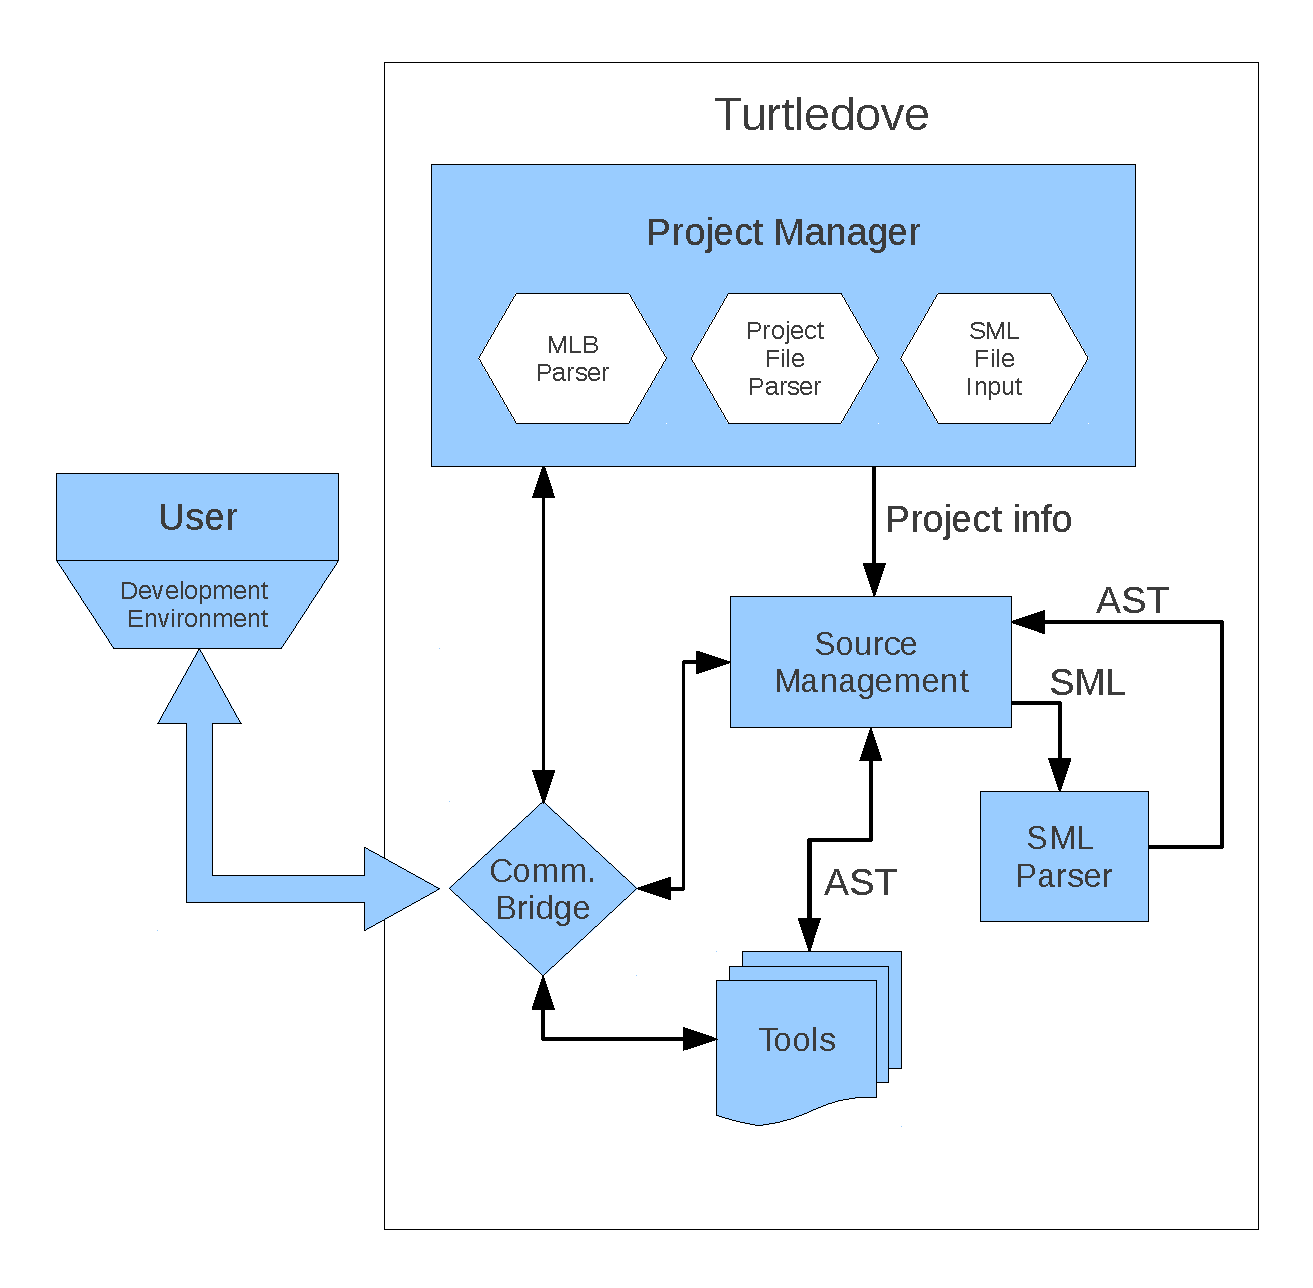
\includegraphics[scale=0.4]{imgs/design/flow.pdf}
  \caption{Design overview of Turtledove and its internal components. Arrows
    symbolise the intercommunication links between internal components.}
  \label{fig:turtledove-design}
\end{figure}

Turtledove consists of two key components (see \fref{fig:turtledove-design}),
the project manager and the rewriting tool. The project manager is an important
part of Turtledove with respect to performance (together with the source
management module) but also to help the novice
programmer in building medium/large programs, whereas the rewriting tool is the
main purpose behind the creation of Turtledove in the first place. Both are
explained in detail below.

\paragraph{Threading}

Threading is an easy way of executing the desired modular design idea of
Turtledove but also as a high throughput is needed by the development
environment. It is of no use if the user has to wait 10+ seconds for auto
completion or looking up the declaration point of a variable because Turtledove
was doing some arbitrary job that had nothing to do with the requested
information. Also it could happen that the user and the development environment
asked for some actions shortly after each other which would otherwise make one
of them wait.

All components within Turtledove including the tools is thus run in a thread for
itself and the communication bridge is used to bind all the threads together.



\subsection{Communication bridge}

The intercommunication links in Turtledove are all controlled by the
communication manager including communication to ``outside'' of Turtledove such
as a development environment. 

% Used below in the cite to refer to the appendix definition of json.
\def \protocoljson {\Fref[plain]{fig:protocol-json}}

The protocol has been chosen to be very simple and versatile with almost no
limitations as it can then be used for both internal and external
communication. The protocol utilises JSON (JavaScript Object
Notation)\cite[\protocoljson]{json} which makes it easy to serialise different types of values
to and from the desired tools inside Turtledove.


\begin{nonfloatingfigure}
{ % so the \angleit command doesn't contaminate the whole environment.
  \newcommand{\angleit}[1]{$\langle$\textnormal{\textit{#1}}$\rangle$}
\begin{lstlisting}
 (@\angleit{request}@) ::= "{ \"Meta\" : (@\angleit{JSON-value}@), \"Dest\" : (@\angleit{JSON-string}@),
                \"Data\" : (@\angleit{JSON-value}@) } \n\n"

(@\angleit{response}@) ::= "{ \"Meta\" : (@\angleit{JSON-value}@), \"Orig\" : (@\angleit{JSON-string}@),
                \"Data\" : (@\angleit{JSON-value}@) } \n\n"
\end{lstlisting}    
}
  
  \caption{Definition of the communication protocol between Turtledove (and its
    tools) and the development evironment.}
  \label{fig:intercom-protocol-def}
\end{nonfloatingfigure}


The protocol is defined (see \fref{fig:intercom-protocol-def}) as a JSON-object
encoded string with two newlines at the end as the stop delimiter. The JSON
object contains three fields, ``Meta'' (Metadata), ``Dest'' (Destination) or
``Orig'' (Origin) and ``Data'' (Data payload) which is described below.

\begin{description}
\item[Meta] is a JSON value specified by the development environment. This value
  is not used in any way by Turtledove but is returned in the response. This
  string is intended for internal bookkeeping by the development environment for
  example to distinguish which file/buffer and/or at which line and column the
  request came from.

  If this feature is not needed by the development environment it can set this
  field to the JSON value \texttt{null} but it is not a requirement.

  Some of the tools may report back when they are done doing something, without
  the development environment has invoked it. In these cases the JSON value
  \texttt{null} will be used.

\item[Dest/Orig] is a non empty JSON string that needs to match a named destination in
  Turtledove. Examples of such a named destinations, also include names of
  tools.
\end{description}


It is important to remember that the resulting string sent to and from
Turtledove must not contain any double newlines except the ones that are defined by
the protocol. This is a requirement, even though the definition of JSON allows
whitespace between a pair of tokens, as it would then render it near to
impossible to determine when the request/response is done without incrementally
parsing the JSON encoded string as it is received.

%%% Local Variables: 
%%% mode: latex
%%% TeX-master: "../../report"
%%% End: 


\subsection{Project manager}
When turtledove is to be used in collaboration with a development environment
and wants to take advantage of all the features it has to offer, the project
manager must be used. The project manager is ultimately responsible for handling
project files which in the end will be converted into an MLB file. 

The reason why project files aren't just MLB files is that they don't enforce
enough limitations in how they are written, which would make it practically
impossible to write a decent tool to manipulate them. Whereas it makes it quite
easy for the user to hack something together.

Dependencies are properly the most challenging thing for a tool to handle as
these may depend on other files and so fourth. 

\begin{example}\ \\
  If we have 3 files: \textit{Foo.sig}, \textit{Foo.sml}, \textit{Main.sml}
  where the \textit{Main.sml} depends on the two \textit{Foo} files and
  obviously \textit{Foo.sml} (implementation) depends on \textit{Foo.sig}
  (signature).

  \begin{sml}
local
  $(SML_LIB)/basis/basis.mlb
  $(SML_LIB)/mylib/MyLib.mlb

  Foo.sig Foo.sml
in
  Main.sml
end    
  \end{sml}
\end{example}

\noindent
From the above example it is practically impossible for a system to know that
\textit{Foo.sml} depends on \textit{Foo.sig} and so forth. It would however be
easy to make up a scheme of how to write MLB files in a ``modular'' way such
that dependencies could be easily processed by a tool, but that would not stop a
user from making valid modifications to the MLB file that would break this
scheme.

Thus we will use a more restricted format for project files but still with the
same functionality as can be expressed in MLB files. See
\fref{sec:appendix-project-manager} for a in depth description of the
functionality.



%%% Local Variables: 
%%% mode: latex
%%% TeX-master: "../../report"
%%% End: 


\subsection{Source management}

Parsing of non well formed code is a major challenge and will always be present
when parsing code that is currently being written. Whether it being a new
function that is currently being written or one or more parts of non well formed
code it will inhibit the SML parser for giving an AST of the entire file. 

Parsing of entire projects is a relative costly operation, the source management
should thus only make the SML parser re parse as small fragments of code as
possible to maintain low response times. 


Multiple steps are taken to make sure these two issues are handled. 

\begin{itemize}
\item Remove non well formed code chunks from the source such that an AST can be
  produced.
  \begin{itemize}
  \item Make sure that position information is not invalid because of any
    temporary removed code in the produced AST
  \item Extract as much information from the non well formed code as possible
    and add this to the environment. For example: In function definitions the
    name and number of arguments could be extracted and added to the environment
    such that syntax colouring of recursive calls can be done and possible error
    reporting of wrong number of arguments in succeeding clauses.
  \end{itemize}

\item Take an old AST, a chunk of code and merge the parsed code into
  the old AST such that a new and update AST is produced.

\item Report errors from the SML parser to the development environment.

\end{itemize}



%%% Local Variables: 
%%% mode: latex
%%% TeX-master: "../../report"
%%% End: 



%
\section{Parsers}

The SML and Rule parsers are both implemented in SML-Lex and SML-Yacc. We say
SML-Lex/Yacc as both the sml/nj version ml-lex/ml-yacc and mlton version
mllex/mlyacc works, but the mosml version mosmllex and mosmlyac are having
problems.

\fixme{fix the above gibberish}

\subsection{Standard ML}

A fine note about whete the grammar was stolen from and possibly some other
clever stuff.

\subsection{Rule}

The Rule parser is based on the SML parser with some added tokens to the lexer
and rules to the grammar to handle the rule syntax (see
\fref{tab:rule-grammar}). 


\subsubsection{Unicode}

The rule syntax uses the symbols \texttt{£} and \texttt{§} to denote
transformers and meta patterns respectively. These were a bit tricky to
implement as they are not ASCII characters. By default SML-Lex\cite{ml-lex-yacc}
only supports 8-bit characters and thus if the upper parts of UTF-8 characters
are needed they must be specially handled. One way to handle it would be to
convert the input file into some fixed length encoding (i.e., UTF-32), but as
SML only uses ASCII chars that would demand a total remake of the Rule lexer
definition. Instead we went with a UTF-8 solution which only need to be
specially fitted for the transformer and meta patterns as it seems that most
editors now a days use UTF-8 as default encoding (seems to be the case for emacs
on linux). Implementing the two UTF-8 values in the lexer was then just a matter
of defining a named expression containing the conjunction of the two decimal
values making up each of the UTF-8 values (see \fref{tab:utf8-rule-values}).

\begin{table}
  \centering
  \begin{tabular}{|l|c|c|c|}
    \hline
    \textbf{Letter} & \textbf{UTF-8} & \textbf{Hex} & \textbf{Decimal} \\ \hline
    Pound sign (£)   & U+00A3 & 0xC2 0xA3 &  $194$ $163$ \\ \hline
    Section sign (§) & U+00A7 & 0xC2 0xA7 & $194$ $167$ \\ \hline
  \end{tabular}

  \caption{Table of UTF-8 and hex values of \texttt{£} and \texttt{§}}
  \label{tab:utf8-rule-values}
\end{table}

As we are using the internal SML-Lex position feature \texttt{yypos} we have to
decrement it by one each time a transformer or meta pattern is encountered as it
is counted as two characters, where it actually is just one (composite)
character.

\subsection{Abstract syntax tree}


%%% Local Variables: 
%%% mode: latex
%%% TeX-master: "../rewriting-syntax"
%%% End: 



\subsection{Tools}

\subsubsection{Rewriting}
...

\subsubsection{Refactoring}
...


etc etc.

%%% Local Variables: 
%%% mode: latex
%%% TeX-master: "../../../report"
%%% End: 




....

%%% Local Variables: 
%%% mode: latex
%%% TeX-master: "../../report"
%%% End: 
